\usepackage{luatexja}
\usepackage[hiragino-pron, nfssonly, deluxe, expert]{luatexja-preset}
\usepackage{fontspec}
\usepackage{epigraph}
\usepackage{etoolbox}
\usepackage{tikz}
\usepackage{framed}
\usepackage{mathtools}
\usepackage{listings}
\usepackage{libertine}
\usepackage[libertine]{newtxmath}
\usepackage{bxcoloremoji}
\usepackage{xcolor}
\usepackage{diagbox}
\usepackage{caption}
\usepackage{appendixnumberbeamer}

\setmonofont{CMU Typewriter Text}

\definecolor{links}{HTML}{2A1B81}
\hypersetup{colorlinks,linkcolor=,urlcolor=links}

\usetheme{Boadilla}
\usecolortheme{seahorse}
% \usefonttheme{serif}

\setbeamercolor{page number in head/foot}{bg=blue!10}
\setbeamertemplate{footline}{%
  \leavevmode%
  \hbox{%
    \begin{beamercolorbox}[wd=.4\paperwidth,ht=2.25ex,dp=1ex,center]{author in head/foot}%
      \usebeamerfont{author in head/foot}\insertshortauthor\hspace*{1ex}(\insertshortinstitute)
    \end{beamercolorbox}%
    \begin{beamercolorbox}[wd=.35\paperwidth,ht=2.25ex,dp=1ex,center]{title in head/foot}%
      \usebeamerfont{title in head/foot}\insertshorttitle
    \end{beamercolorbox}%
    \begin{beamercolorbox}[wd=.15\paperwidth,ht=2.25ex,dp=1ex,center]{date in head/foot}%
      \insertshortdate
    \end{beamercolorbox}%
    \begin{beamercolorbox}[wd=.1\paperwidth,ht=2.25ex,dp=1ex,center]{page number in head/foot}%
      \insertframenumber{} / \inserttotalframenumber\hspace*{1ex}
    \end{beamercolorbox}}%
  \vskip0pt%
}

\beamertemplatenavigationsymbolsempty

\setbeamertemplate{bibliography item}{\insertbiblabel}
\setbeamersize{description width=1cm}
\setbeamertemplate{items}[circle]
\setbeamertemplate{section in toc}[circle]
\setbeamertemplate{subsection in toc}{%
  \leavevmode\leftskip=2em
  {%
    \usebeamerfont*{itemize item}%
    \usebeamercolor{subsection number projected}%
    \color{bg}%
    \raise1.25pt\hbox{\donotcoloroutermaths$\bullet$}}%
  \hskip1.5ex\inserttocsubsection\par}

% Definitions for the title page
\newcommand*{\GitHub}[1]{%
  \gdef\InsertGitHub{#1}%
}
\newcommand*{\Email}[1]{%
  \gdef\InsertEmail{\href{mailto:#1}{#1}}%
}
\newcommand*{\Conference}[1]{%
  \gdef\InsertConference{#1}%
}
\setbeamerfont{title}{size=\huge, series=\bfseries, family=\mcfamily\rmfamily}
\setbeamercolor{title}{bg=white}
\setbeamerfont{email}{size=\scriptsize, family=\ttfamily}
\setbeamercolor{email}{bg=white}
\setbeamerfont{date}{shape=\itshape, family=\rmfamily}
\setbeamerfont{vc}{size=\scriptsize, family=\ttfamily}
\setbeamercolor{vc}{bg=white}

\input{vc.tex}

\setbeamertemplate{title page}
{%
  \vbox{}
  \vfill
  \begingroup
    \centering
    \hrulefill
    \vskip1em\par
    \begin{beamercolorbox}[sep=8pt,center,shadow=false,rounded=true]{title}
      \usebeamerfont{title}\inserttitle\par%
      \ifx\insertsubtitle\@empty%
      \else%
        \vskip0.25em%
        {\usebeamerfont{subtitle}\usebeamercolor[fg]{subtitle}\insertsubtitle\par}%
      \fi%     
    \end{beamercolorbox}%
    \hrulefill
    \vskip1em\par
    \begin{beamercolorbox}[sep=0pt,center,shadow=false,rounded=true]{author}
      \usebeamerfont{author}\insertauthor
    \end{beamercolorbox}
    \begin{beamercolorbox}[sep=0pt,center,shadow=false,rounded=true]{email}
      \usebeamerfont{email}\InsertEmail
    \end{beamercolorbox}
    \vskip1em
    \begin{beamercolorbox}[sep=5pt,center,shadow=false,rounded=true]{institute}
      \usebeamerfont{institute}\insertinstitute
    \end{beamercolorbox}
    \begin{beamercolorbox}[sep=5pt,center,shadow=false,rounded=true]{date}
      \usebeamerfont{date}\insertdate @ \InsertConference
    \end{beamercolorbox}
    \begin{beamercolorbox}[sep=0pt,center,shadow=false,rounded=true]{vc}
      \usebeamerfont{vc}
      \href{https://github.com/\InsertGitHub}{%
        \InsertGitHub@\GITAbrHash%
      }%
    \end{beamercolorbox}\vskip0.5em
    {\usebeamercolor[fg]{titlegraphic}\inserttitlegraphic\par}
  \endgroup
  \vfill
}
\setbeamertemplate{blocks}[rounded][shadow=false]
\setbeamertemplate{note page}{\pagecolor{yellow!5}\insertnote}


% ============ ここを消すとNote消える ================
% \mode<handout>{%
%   \setbeameroption{show notes on second screen=right}%
% }
% ============ ここを消すとNote消える ================


\renewcommand{\kanjifamilydefault}{\gtdefault}

\resetcounteronoverlays{lstlisting}
\definecolor{bluegray}{rgb}{0.4, 0.6, 0.8}
\DeclareCaptionFormat{listing}{{\color{bluegray}\lstlistingname}#2#3}
\captionsetup[lstlisting]{format=listing, font={footnotesize}}

\setmonofont[Ligatures=TeX]{CMU Typewriter Text}

\setbeamertemplate{items}[circle]

\newfontfamily\quotefont[Ligatures=TeX]{Linux Libertine O} % selects Libertine as the quote font

\newcommand*\quotesize{60} % if quote size changes, need a way to make shifts relative
% Make commands for the quotes
\newcommand*{\openquote}
   {\tikz[remember picture,overlay,xshift=-4ex,yshift=-2.5ex]
   \node (OQ) {\quotefont\fontsize{\quotesize}{\quotesize}\selectfont``};\kern0pt}

\newcommand*{\closequote}[1]
  {\tikz[remember picture,overlay,xshift=1.5ex,yshift={#1}]
   \node (CQ) {\quotefont\fontsize{\quotesize}{\quotesize}\selectfont''};}

\newcommand*\shadedauthorformat{\emph} % define format for the author argument

% Now a command to allow left, right and centre alignment of the author
\newcommand*\authoralign[1]{%
  \if#1l
    \def\authorfill{}\def\quotefill{\hfill}
  \else
    \if#1r
      \def\authorfill{\hfill}\def\quotefill{}
    \else
      \if#1c
        \gdef\authorfill{\hfill}\def\quotefill{\hfill}
      \else\typeout{Invalid option}
      \fi
    \fi
  \fi}
% wrap everything in its own environment which takes one argument (author) and one optional argument
% specifying the alignment [l, r or c]
%
\newenvironment{shadequote}[2][l]%
{\authoralign{#1}
\ifblank{#2}
   {\def\shadequoteauthor{}\def\yshift{-2ex}\def\quotefill{\hfill}}
   {\def\shadequoteauthor{\par\authorfill\shadedauthorformat{#2}}\def\yshift{2ex}}
\begin{quote}\normalfont\openquote}
{\shadequoteauthor\quotefill\closequote{\yshift}\end{quote}}

\makeatletter
\def\@fnsymbol#1{\ensuremath{\ifcase#1\or *\or \dagger\or \ddagger\or
   \mathsection\or \mathparagraph\or \|\or **\or \dagger\dagger
   \or \ddagger\ddagger \else\@ctrerr\fi}}
\makeatother

\renewcommand{\thefootnote}{\fnsymbol{footnote}}

\newcommand\ballcircle[1]{%
  {%
    \usebeamercolor{enumerate item}%
    \tikzset{beameritem/.style={circle,inner sep=0,minimum size=2ex,text=enumerate item.bg,fill=enumerate item.fg,font=\footnotesize}}%
    \tikz[baseline=(n.base)]\node(n)[beameritem]{#1};%
  }
}
\newcommand\ballref[1]{%
  \ballcircle{\ref{#1}}
}

\usetikzlibrary{calc}
\usetikzlibrary{shapes.callouts} 

\pgfkeys{%
    /calloutquote/.cd,
    width/.code                   = {\def\calloutquotewidth{#1}},
    position/.code                = {\def\calloutquotepos{#1}}, 
    author/.code                  = {\def\calloutquoteauthor{#1}},
    at/.code                      = {\def\calloutquoteat{#1}},
    sign/.code                    = {\def\calloutquotesign{#1}},
    /calloutquote/.unknown/.code  = {\let\searchname=\pgfkeyscurrentname
                                      \pgfkeysalso{\searchname/.try=#1,                        
                                      /tikz/\searchname/.retry=#1},\pgfkeysalso{\searchname/.try=#1,
                                      /pgf/\searchname/.retry=#1}
                                    }
}

\makeatletter

\newsavebox\temp@simple@callout@author@box
\newcommand\calloutquote[2][]{%
  \pgfkeys{/calloutquote/.cd,
    width    = 5cm,
    position = {(0.5,-0.2)},
    at       = {(0,0)},
    author   = {},
    sign     = {+}
  }%
  \pgfqkeys{/calloutquote}{#1}%
  \sbox{\temp@simple@callout@author@box}{\mbox{%
    \begin{tabular}{l}
      \calloutquoteauthor%
    \end{tabular}
  }}%
  \node [rectangle callout,callout relative pointer={\calloutquotepos},text width=\calloutquotewidth,/calloutquote/.cd,
     #1] (tmpcall) at \calloutquoteat {\hfil#2\hfil};
  \node at ($ (tmpcall.pointer) - (-\calloutquotesign0.5\wd\temp@simple@callout@author@box,0.7\ht\temp@simple@callout@author@box) $) {\calloutquoteauthor};
}

\newsavebox\temp@simple@callout@box
\newcommand{\simplecallout}[4][{}]{%
  \sbox{\temp@simple@callout@box}{\mbox{%
    \begin{tabular}{l}
      #4%
    \end{tabular}
  }}%
  \begin{center}%
    \begin{tikzpicture}%
      \calloutquote[width=1.05\wd\temp@simple@callout@box,position={(#2.5,-0.2)},fill=#3,rounded corners,author={#1},sign=#2]{
        #4%
      }%
    \end{tikzpicture}%
  \end{center}
}

\makeatother
\newfontfamily\listingfont{Menlo}
\definecolor{dkgreen}{rgb}{0,0.6,0}
\definecolor{gray}{rgb}{0.5,0.5,0.5}
\definecolor{mauve}{rgb}{0.58,0,0.82}

\makeatletter
\lst@CCPutMacro\lst@ProcessOther {"2D}{\lst@ttfamily{-{}}{-{}}}
\@empty\z@\@empty
\makeatother

\lstdefinestyle{csharp}{
  numbers=left,
  language=[Sharp]C
}

\lstdefinestyle{cil}{
  numbers=left,
  language=CIL
}

\lstdefinestyle{plain}{
  basicstyle=\listingfont\tiny,
  language=
}

\lstdefinestyle{sh}{
  numbers=left,
  language=sh
}

\lstdefinestyle{c}{
  numbers=left,
  language=C
}

\lstdefinestyle{python}{
  numbers=left,
  language=Python
}

\lstdefinestyle{asm-x86}{
  numbers=left
}

\lstdefinestyle{pseudo-code}{
  numbers=left,
  keywords=[6]{for,from,to,endfor,while,endwhile}
}

\lstdefinestyle{bitcoin-script}{
  mathescape=true
}

\lstset{
  basicstyle=\listingfont,
  frame=single,
  xleftmargin=2em,
  xrightmargin=1em,
  breaklines=true
}

\lstdefinestyle{scala}{
  basicstyle=\listingfont\scriptsize,
  breakatwhitespace=false,
  language=scala,
  captionpos=b,
  commentstyle=\listingfont\scriptsize\color{dkgreen},
  extendedchars=true,
  xleftmargin=1em,
  xrightmargin=1em,
  keepspaces=true,
  keywordstyle=\listingfont\scriptsize\color{blue},
  emphstyle=\listingfont\scriptsize\color{cyan},
  rulecolor=\listingfont\scriptsize\color{black},
  showspaces=false,
  showstringspaces=false,
  showtabs=false,
  stringstyle=\listingfont\scriptsize\color{mauve},
  tabsize=2
}

\lstdefinelanguage{scala}{
  morekeywords={abstract,case,catch,class,def,%
    do,else,extends,false,final,finally,%
    for,if,implicit,import,match,mixin,%
    new,null,object,override,package,%
    private,protected,requires,return,sealed,%
    super,this,throw,trait,true,try,%
    type,val,var,while,with,yield},
  moreemph={Byte,Short,Int,Long,Float,Double,Char,
    String,Boolean,Unit,Null,Nothing,Any,AnyRef,
    Left,Right,Either},
  otherkeywords={=>,<-,<\%,<:,>:,\#,@},
  sensitive=true,
  morecomment=[l]{//},
  morecomment=[n]{/*}{*/},
  morestring=[b]",
  morestring=[b]',
  morestring=[b]"""
}

\lstdefinestyle{go}{
  basicstyle=\listingfont\scriptsize,
  breakatwhitespace=false,
  language=go,
  captionpos=b,
  commentstyle=\listingfont\scriptsize\color{dkgreen},
  extendedchars=true,
  xleftmargin=1em,
  xrightmargin=1em,
  keepspaces=true,
  keywordstyle=\listingfont\scriptsize\color{blue},
  emphstyle=\listingfont\scriptsize\color{cyan},
  rulecolor=\listingfont\scriptsize\color{black},
  showspaces=false,
  showstringspaces=false,
  showtabs=false,
  stringstyle=\listingfont\scriptsize\color{mauve},
  tabsize=2
}


\lstdefinelanguage{golang}%
  {morekeywords=[1]{package,import,func,type,struct,return,defer,panic,%
     recover,select,var,const,iota},%
   morekeywords=[2]{string,uint,uint8,uint16,uint32,uint64,int,int8,int16,%
     int32,int64,bool,float32,float64,complex64,complex128,byte,rune,uintptr,%
     error,interface},%
   morekeywords=[3]{map,slice,make,new,nil,len,cap,copy,close,true,false,%
     delete,append,real,imag,complex,chan,},%
   morekeywords=[4]{for,break,continue,range,go,goto,switch,case,fallthrough,if,%
     else,default,},%
   morekeywords=[5]{Println,Printf,Error,Print,},%
   sensitive=true,%
   morecomment=[l]{//},%
   morecomment=[s]{/*}{*/},%
   morestring=[b]',%
   morestring=[b]",%
   morestring=[s]{`}{`},%
}

\newcommand\ce[1]{%
  \coloremojiucs{#1}
}

\newenvironment{notes}
  {%
    \begin{xlrbox}{NotesBox}
    \begin{minipage}{.95\textwidth}
    \small\rmfamily\mcfamily
    \begin{itemize}
    \setlength{\itemindent}{0em}
  }{%
    \end{itemize}
    \end{minipage}
    \end{xlrbox}
    \note{\theNotesBox}}

\title{Featherweight Goをつくる}
\author[Yoshimura Hikaru]{%
  \textsc{Yoshimura} Hikaru(吉村 優)
}
\Email{hikaru\_yoshimura@r.recruit.co.jp}
\date[July 17, 2020]{%
  \oldstylenums{July 17, 2020}
}
\Conference{Quipper LT}
\institute[\InsertEmail]{%
  Englishバックエンド開発グループ
}
\GitHub{y-yu/featherweight\_go-slide}

\begin{document}

\frame{\maketitle}

\begin{frame}
  \frametitle{目次}

  \tableofcontents
\end{frame}

\section{自己紹介}
\begin{frame}
  \frametitle{自己紹介}
  
  \begin{columns}
    \begin{column}{0.22\textwidth}
      \begin{center}
        \begin{figure}[h]
          
\includegraphics[width=0.95\textwidth]{img/bird2x.png}%
        \end{figure}
      \end{center}
 
      \begin{table}[h]
        \begin{tabular}{ll}
          Twitter & \href{https://twitter.com/\_yyu\_}{@\_yyu\_} \\
          Qiita &  \href{https://qiita.com/yyu}{yyu} \\
          GitHub &  \href{https://github.com/y-yu}{y-yu} \\
          Facebook & \href{https://www.facebook.com/h1karuy}{h1karuy} \\
        \end{tabular}
      \end{table}
    \end{column}
    \begin{column}{0.78\textwidth}
      \pause
      \begin{itemize}
        \item 筑波大学 情報学群情報科学類卒(学士)
        \begin{itemize}
          \item 正規表現を利用した型システムの研究
        \end{itemize}

        \item 株式会社リクルートマーケティングパートナーズ(中途)
        \begin{itemize}
          \item スタディサプリENGLISH サーバーサイド(Scala)
        \end{itemize}

        \item 未踏ターゲット事業(ゲート式量子コンピュータ)
        \begin{itemize}
          \item 公平な抽選プロトコルの開発・シミュレーター実装
        \end{itemize}

        \item 暗号・セキュリティー
        \begin{itemize}
          \item 大学同期とのチームでCTF活動を7年くらいやっている
        \end{itemize}

        \item {\LaTeX}組版
        \begin{itemize}
          \item 同人誌を5年くらい作っている
          \item \href{https://github.com/rust-lang-ja/book-ja-pdf}{The Rust Programming Language 2nd Edition(日本語)}や
          \href{https://github.com/ymotongpoo/erlang-in-anger}{Erlang in Anger(日本語)}の組版をやった
          \item このスライドも全部{\LaTeX}で作った
        \end{itemize}
      \end{itemize}
    \end{column}
  \end{columns}
\end{frame}

\section{Featherweight Goとは?}

\begin{frame}
  \frametitle{Featherweight Goとは}

  \pause
  \begin{itemize}
    \item<+-> Featherweight Go(FG)は\cite{griesemer2020featherweight}で導入された
    Go言語から``Goの特徴''を残した最小の部分を取り出した小型モデル言語

    \item<+-> Go言語は実用言語なので、フォーマルな議論などには不要な機能がある
    (たとえばシンタックスシュガーとか)

    \item<+-> 実用するには不便ではあるが、FGでGo言語が表現できるなら、
    FGで型などの議論をすればよく、考えることが減る

    \item<+-> 似たようなコンセプトに\emph{Featherweight Java}\cite{10.1145/503502.503505}や
    \emph{DOT}\cite{Amin:215280}がある

    \item<+-> 本来は型システムなどの形式手法を議論するためのものだが、
    小さいので自作するのが楽ということでやってみた
  \end{itemize}
\end{frame}

\begin{frame}
  \frametitle{Featherweight Goとは}

  \begin{itemize}
    \item<+-> \cite{griesemer2020featherweight}では
    さらに\emph{Generics}を入れた
    ``FGG''(Featherweight Go with Generics)を定義している

    \item<+-> そしてFGGからFGへの変換(\emph{monomorphisation})を定義することで、
    \begin{enumerate}
      \item Go言語のコードはFGのコードで(量は増えるけど)表現できる
      \item 型が付くFGGのコードを、型がつくFGへ変換できる
      \item したがってFG経由でGo言語にGenericsが入れられる
    \end{enumerate}

    \item<+-> まだFGGは実装してない\ce{:innocent:}ので、
    FGだけについて今回は解説!
 \end{itemize}
\end{frame}

\begin{frame}[fragile]
  \frametitle{Featherweight Goの機能}

  \pause
  \begin{itemize}
    \item<+-> 機能を列挙すると\ce{:point_down}となる
    \begin{itemize}
      \item プリミティブ型はなし(!?)

      \item \lstinline|struct|(構造体)と\lstinline|interface|(インターフェース)の宣言

      \item 関数定義

      \item 構造体の初期化・フィールド解決

      \item メソッドコール
    \end{itemize}

    \uncover<+->{%
      \simplecallout[%
        {
\includegraphics[width=0.1\textwidth]{img/hacker_angry.png}}
        ]{+}{red!10}{これじゃ使い物にならんでしょ\ce{:rage:}}
    }

    \item<+-> とはいえこれくらいあれば、実はそれなりなものが書ける

    \item<+-> \url{https://y-yu.github.io/featherweight_go/}
    \ce{:point_left:}で今すぐ試そう!
  \end{itemize}
\end{frame}


\begin{frame}[fragile]
  \frametitle{Featherweight Goのプログラム例}

  \begin{columns}
    \begin{column}{0.6\textwidth}
\begin{lstlisting}[style=go]
package main;

type Nat interface {
  plus(a Nat) Nat
}

type Zero struct { }
type Succ struct {
  pred Nat
}

func (this Zero) plus(a Nat) Nat {
  return a
}
func (this Succ) plus(a Nat) Nat {
  return Succ{this.pred.plus(a)}
}

func main() {
  _ = Succ{Succ{Zero{}}}.plus(Succ{Succ{Zero{}}})
}
\end{lstlisting}
    \end{column}
    \begin{column}{0.4\textwidth}
      \pause
      \begin{description}
        \item[\texttt{Zero}] $0$を定義
        \item[\texttt{Succ(n)}] $n + 1$を定義
      \end{description}

      \pause
      \simplecallout[%
        {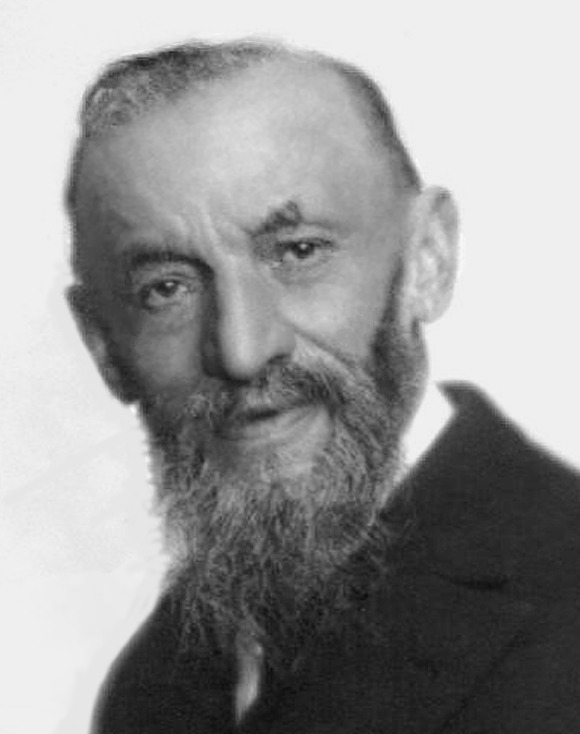
\includegraphics[width=0.15\textwidth]{img/Peano.jpg}}
      ]{-}{green!10}{自然数の完成!}

      \pause
      \begin{itemize}
        \item<+-> \lstinline|Succ{Succ{Zero{}}}|は$1 + 1 + 0 = 2$

        \item<+-> $2 + 2$となり結果は$4$を表わす\ce{:point_down}となる
        \begin{lstlisting}[style=plain]
Succ{Succ{Succ{Succ{Zero{}}}}}
        \end{lstlisting}
      \end{itemize}
    \end{column}
  \end{columns}
\end{frame}


\section{プログラム言語処理系をつくるには?}

\begin{frame}
  \frametitle{プログラム言語処理系をつくるには?}

  \pause
  \begin{itemize}
    \item<+-> 言語処理系はだいたい次の流れになる
    \begin{description}
      \item[1. パーズ] 文字列レベルのコード(具象構文)を\textbf{抽象構文木}へ変換する
      \item[2. 型チェック] 抽象構文木に型が付くかを検査する
      \item[3. 実行] 抽象構文木に基づいてプログラムを実行する
    \end{description}
  \end{itemize}

  \uncover<+->{
    \simplecallout[%
      {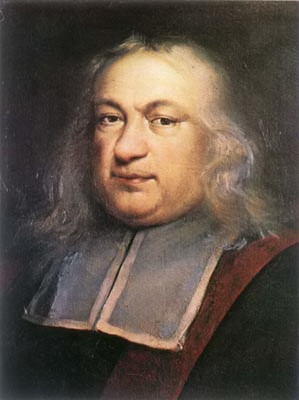
\includegraphics[width=0.08\textwidth]{img/Fermat.jpg}}
    ]{-}{red!10}{この余白はそれを書くには狭すぎる}
  }

  \uncover<+->{
    \simplecallout[%
      {
\includegraphics[width=0.08\textwidth]{img/yoshi.jpg}}
    ]{+}{cyan!10}{すごい雑に説明するか!}
  }
\end{frame}

\section{Featherweight Goの実装}

\begin{frame}
  \frametitle{パーザーの作成}

  \pause
  \simplecallout{-}{gray!10}{\huge\bfseries \ce{:punch:}\mbox{!!!}気合!!!\ce{:punch:}}

  \pause
  \begin{itemize}
    \item<+-> 具象構文から抽象構文にするのが辛すぎる……\ce{:innocent:}
    \begin{itemize}
      \item いちおう正規表現エンジンを自作した経験があるけど、それでもつらい
    \end{itemize}

    \item<+-> 詳細はとにかく面倒なので\textbf{全て割愛}します!

    \item<+-> さっきの3つの中でパーザーが最も面倒だと思う
    \begin{itemize}
      \item このスライド作ってる間にもバグを見つけた……
    \end{itemize}

    \item<+-> プログラム言語を作りたいけどパーザーに興味はないなら、
    具象構文としてJSONなどを使ってしまうという手もある……\ce{:thinking:}
  \end{itemize}
\end{frame}

\begin{frame}
  \frametitle{型検査器の作成}

  \begin{columns}
    \begin{column}{0.4\textwidth}
      \begin{figure}
        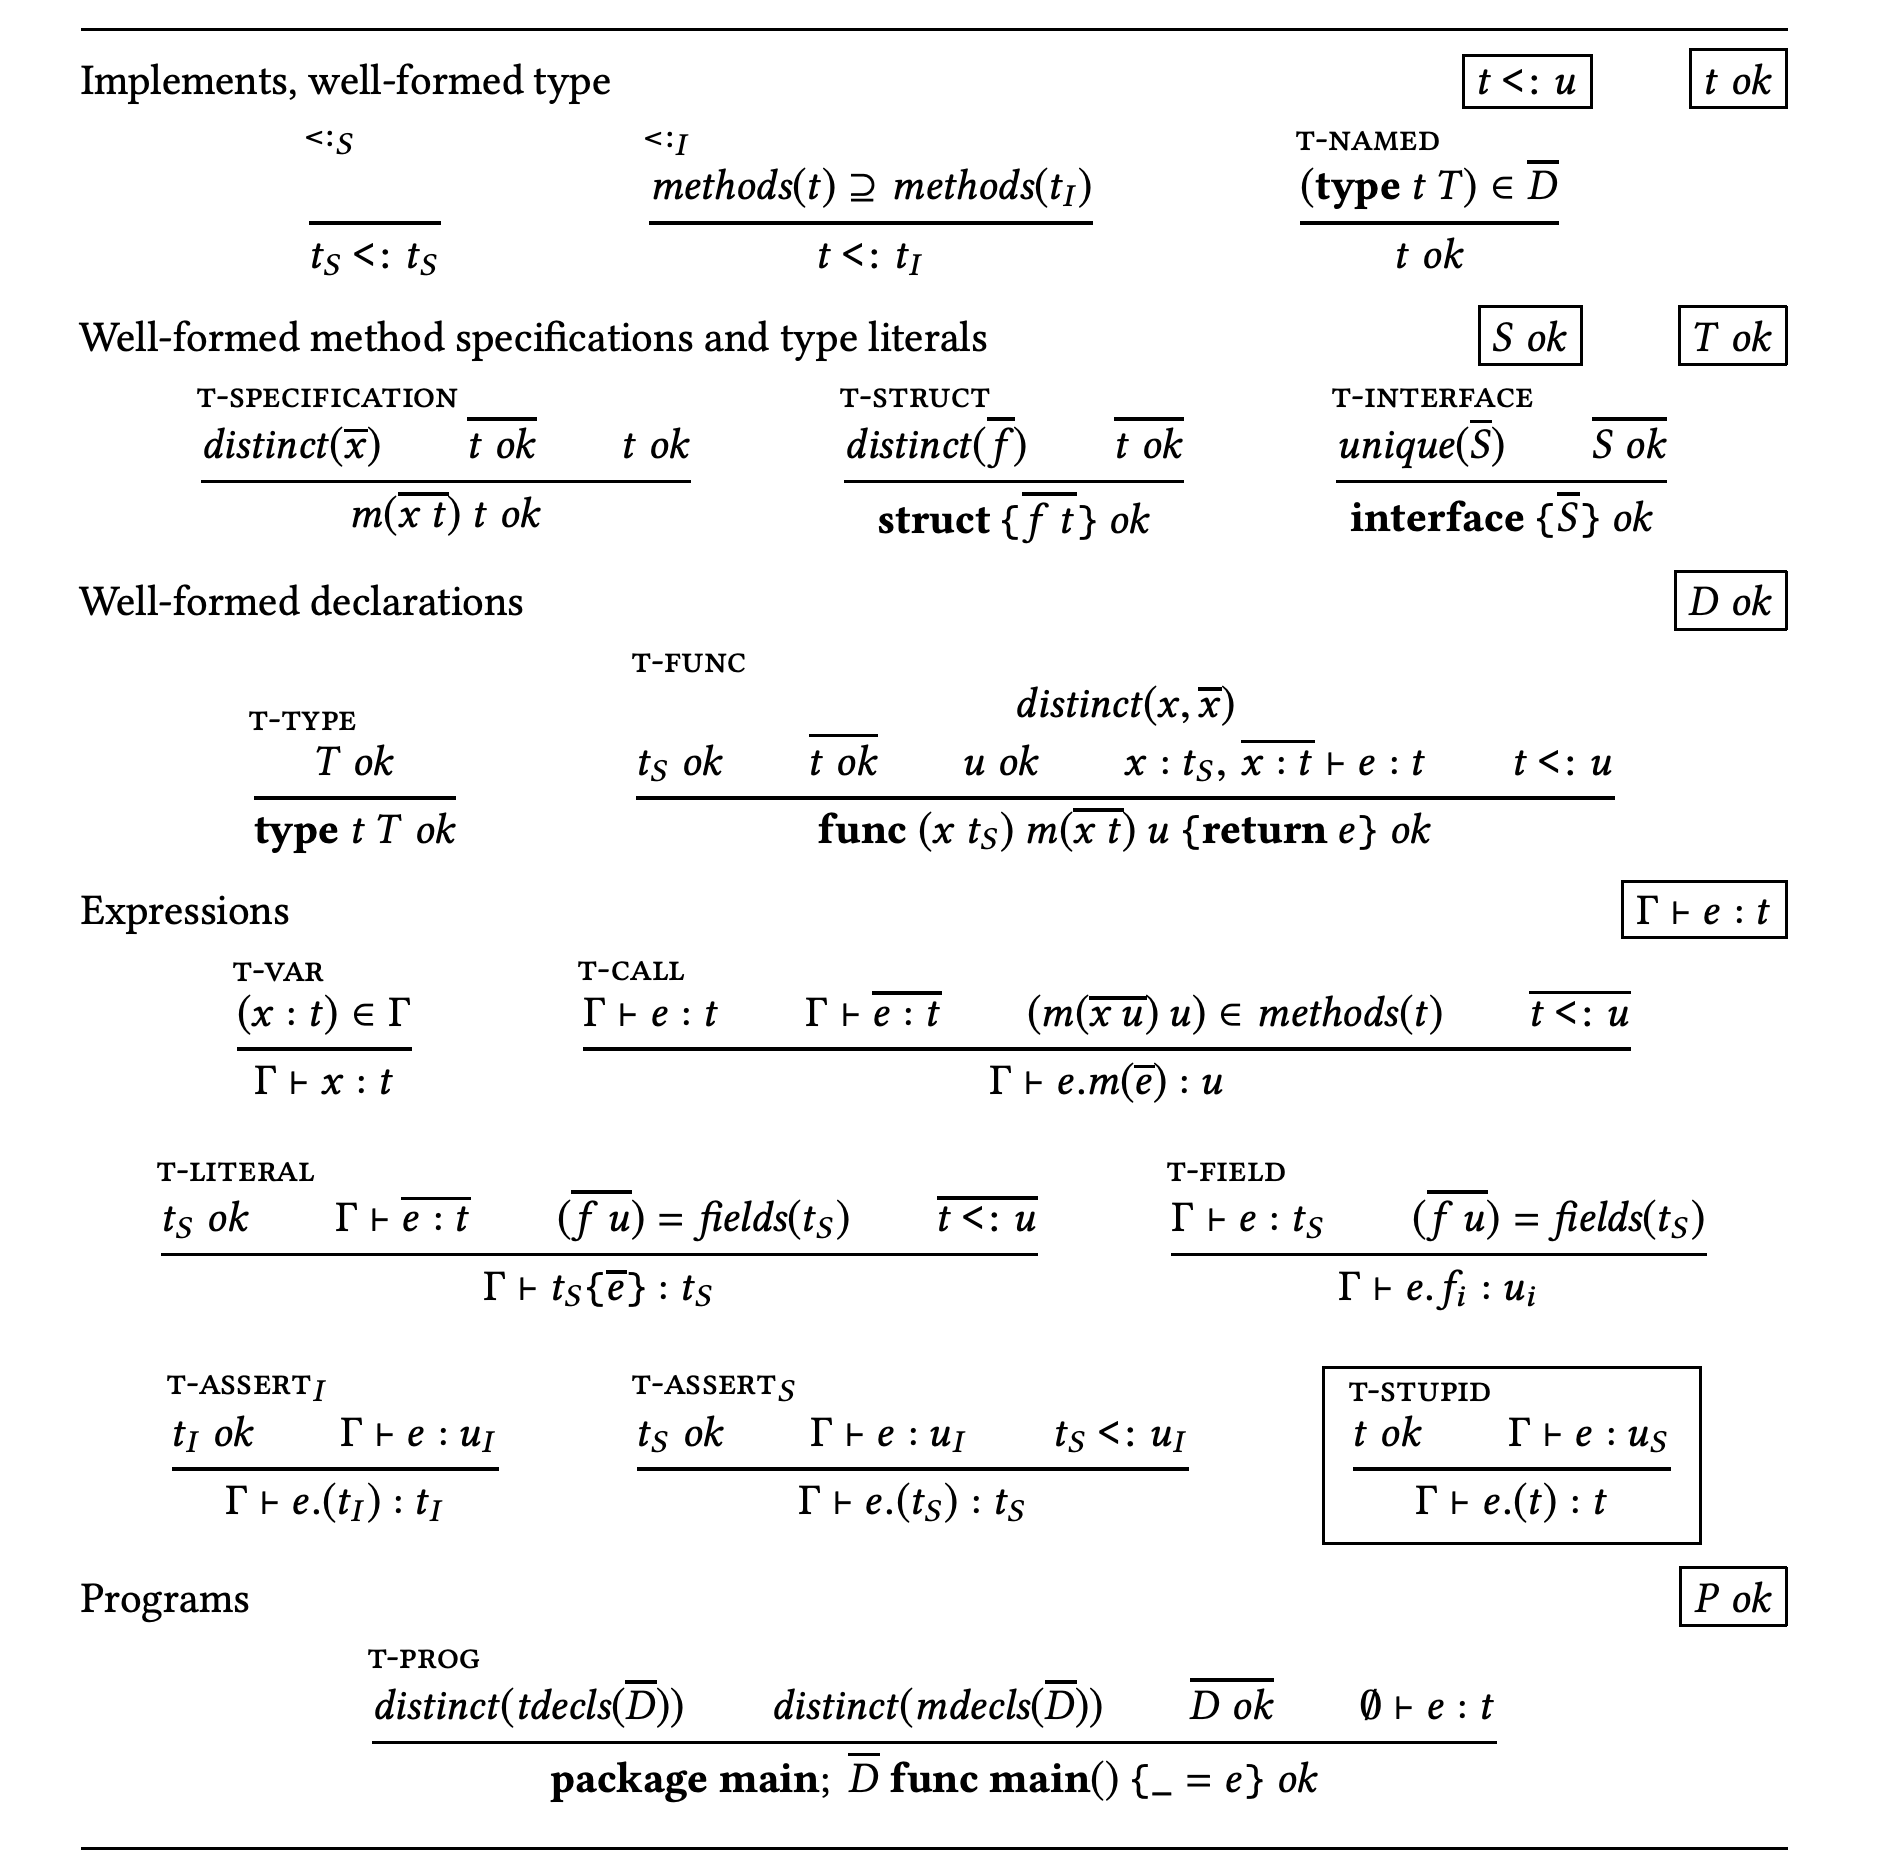
\includegraphics[width=\textwidth]{img/type_rule.png}
        \caption{\cite{griesemer2020featherweight}より}
      \end{figure}
    \end{column}
    \begin{column}{0.6\textwidth}
      \pause
      \begin{itemize}
        \item<+-> \ce{:point_left:}型ルールの図に基づいて、ひたすら実装

        \uncover<+->{%
          \simplecallout[%
            {
\includegraphics[width=0.1\textwidth]{img/phone_cat.png}}
          ]{+}{blue!10}{なにこれ?}
        }

        \item<+-> 読めるようになると、英語(論文)が読めなくても
        ある程度なんとかなる(?)

        \uncover<+->{%
          \simplecallout[%
            {
\includegraphics[width=0.15\textwidth]{img/tapl.png}}
          ]{-}{red!10}{日本語で学べます!}
        }
      \end{itemize}
    \end{column}
  \end{columns}
\end{frame}

\begin{frame}
  \frametitle{評価器の作成}

  \pause
  \begin{itemize}
    \item<+-> \ce{:point_down:}評価ルール(意味論)の図に基づいて、ひたすら実装
  \end{itemize}

  \begin{columns}
    \begin{column}{0.65\textwidth}
      \begin{figure}
        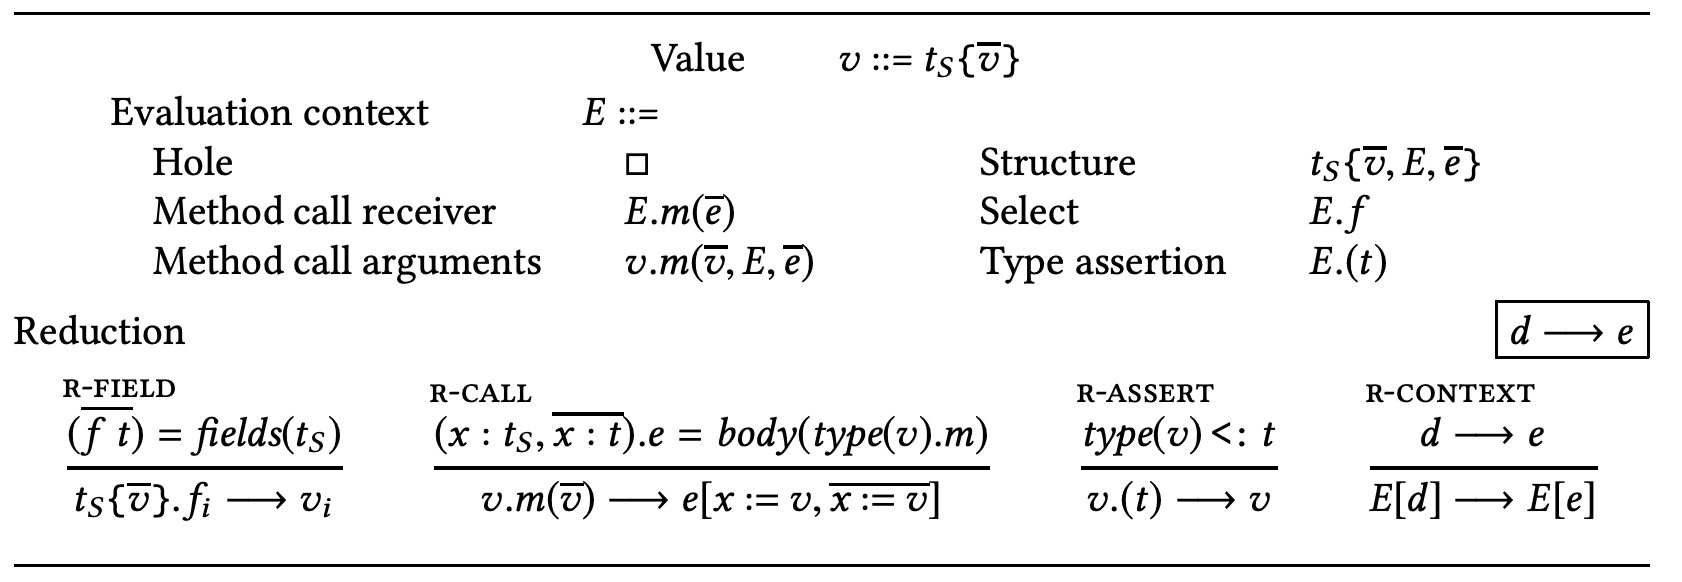
\includegraphics[width=\textwidth]{img/eval_rule.png}
        \caption{\cite{griesemer2020featherweight}より}
      \end{figure}
    \end{column}
    \begin{column}{0.35\textwidth}
      \simplecallout[%
        {
\includegraphics[width=0.2\textwidth]{img/phone_cat.png}}
      ]{-}{blue!10}{どうして?}

      \uncover<+->{%
        \simplecallout[%
          {
\includegraphics[width=0.2\textwidth]{img/tapl.png}}
        ]{+}{red!10}{日本語で学べます!}
      }
    \end{column}
  \end{columns}
\end{frame}


\begin{frame}
  \frametitle{Webアプリ}

  \begin{columns}
    \begin{column}{0.5\textwidth}
      \pause
      \simplecallout[%
        {
\includegraphics[width=0.12\textwidth]{img/bird2x.png}}
      ]{-}{cyan!10}{\emph{Scala.js}{\footnotemark}で簡単に \\
        Webアプリにならないかな\ce{:thinking:}}

      \pause
      \simplecallout[%
        {
\includegraphics[width=0.12\textwidth]{img/xuwei.png}}
      ]{+}{green!10}{\large できそう}
    \end{column}
    \begin{column}{0.5\textwidth}
      \begin{itemize}
        \item \ce{:point_left:}というようなノリで
        Scala.jsでWebアプリとなった!\ce{:tada:}
       
        \item Web UIの作り方が分からなさすぎたけど、
        \texttt{@nanashiki, @kazuma1989, @nobuoka}の助けでどうにか完成\ce{:pray:}
      \end{itemize}
      
      \footnotetext{\url{https://www.scala-js.org/}}
    \end{column}
  \end{columns}

  \pause
  \begin{shadequote}{}
    \begin{center}
      あなたとFeatherweight Go、いますぐダウンロード(?)

      \url{https://y-yu.github.io/featherweight_go/}
    \end{center}
  \end{shadequote}
\end{frame}

\section{まとめ}
\begin{frame}
  \frametitle{まとめ}

  \pause
  \begin{itemize}
    \item<+-> こんな感じでFeatherweight Goができた(?)
    \begin{itemize}
      \item \url{https://github.com/y-yu/featherweight_go}
    \end{itemize}

    \item<+-> (ほぼ全て割愛したけど)実はパーザーを除いて、他はすごくシンプルにできた

    \item<+-> 教科書に載っていない言語をちょっと作ってみたくなったときにおすすめ

    \item<+-> FGGもそのうち作りたい

    \uncover<+->{
      \simplecallout[%
        {
\includegraphics[width=0.1\textwidth]{img/computer_programming_man.png}}
      ]{-}{orange!10}{Go言語にGenericsを入れるとコンパイルが遅くなるのでは……?}
    }

    \item<+-> そういうこと\ce{:point_up:}を思ったら、ぜひ
    FGGを実装してみましょう!

    \item<+-> だいたいのことはTaPL(日本語)\cite{BB12112636}に載っています
  \end{itemize}
\end{frame}

\section*{参考文献}

\begin{frame}[allowframebreaks]
  \frametitle{参考文献}

  \bibliographystyle{junsrt_url}
  \bibliography{ref}
\end{frame}

\begin{frame}
  \centering
  {\Huge Thank you for your attention!}
\end{frame}

\end{document}
